% Workflow_Overview.tex — Claude Code Academic Workflow
% Compile: xelatex → bibtex → xelatex → xelatex
\documentclass[10pt, aspectratio=169]{beamer}
% header.tex — Shared Beamer preamble
% Theme: metropolis | Engine: XeLaTeX | Bib: bibtex

% ----------------------------------------------------------------------
% Theme and fonts
% ----------------------------------------------------------------------
\usetheme{metropolis}
\metroset{
  progressbar=frametitle,
  numbering=fraction,
  block=fill,
  sectionpage=progressbar
}

% ----------------------------------------------------------------------
% Colors
% ----------------------------------------------------------------------
\definecolor{NavyPrimary}{HTML}{1B2A4A}
\definecolor{TealAccent}{HTML}{2E7D8C}
\definecolor{GoldAlert}{HTML}{D4A843}
\definecolor{LightGold}{HTML}{FDF6E3}
\definecolor{LightTeal}{HTML}{E8F4F6}
\definecolor{LightGray}{HTML}{F5F5F5}

\setbeamercolor{palette primary}{bg=NavyPrimary}
\setbeamercolor{frametitle}{bg=NavyPrimary}
\setbeamercolor{title separator}{fg=TealAccent}
\setbeamercolor{progress bar}{fg=TealAccent, bg=NavyPrimary!20}
\setbeamercolor{alerted text}{fg=GoldAlert}
\setbeamercolor{example text}{fg=TealAccent}

% ----------------------------------------------------------------------
% Packages
% ----------------------------------------------------------------------
\usepackage{booktabs}
\usepackage{tabularx}
\usepackage{tikz}
\usetikzlibrary{
  arrows.meta,
  positioning,
  shapes.geometric,
  fit,
  calc,
  backgrounds
}
\usepackage[most]{tcolorbox}
\usepackage{fontawesome5}
\usepackage{listings}
\usepackage{graphicx}
\usepackage{hyperref}

% ----------------------------------------------------------------------
% Listings style
% ----------------------------------------------------------------------
\lstset{
  basicstyle=\ttfamily\scriptsize,
  backgroundcolor=\color{LightGray},
  frame=none,
  breaklines=true,
  columns=fullflexible,
  keepspaces=true,
  xleftmargin=4pt,
  xrightmargin=4pt
}

% ----------------------------------------------------------------------
% Custom tcolorbox environments
% ----------------------------------------------------------------------

% keybox — Gold background for key takeaways
\newtcolorbox{keybox}{
  colback=LightGold,
  colframe=GoldAlert,
  boxrule=0.5pt,
  arc=2pt,
  left=6pt, right=6pt,
  top=4pt, bottom=4pt,
  fontupper=\small
}

% highlightbox — Teal left-accent for highlights
\newtcolorbox{highlightbox}{
  colback=LightTeal,
  colframe=TealAccent,
  boxrule=0pt,
  borderline west={3pt}{0pt}{TealAccent},
  arc=0pt,
  left=8pt, right=6pt,
  top=4pt, bottom=4pt,
  fontupper=\small
}

% definitionbox — Navy titled box for definitions
\newtcolorbox{definitionbox}[1][Definition]{
  colback=white,
  colframe=NavyPrimary,
  boxrule=1pt,
  arc=2pt,
  title=#1,
  fonttitle=\bfseries\small,
  fontupper=\small,
  coltitle=white,
  colbacktitle=NavyPrimary,
  left=6pt, right=6pt,
  top=4pt, bottom=4pt
}

% ----------------------------------------------------------------------
% Utility commands
% ----------------------------------------------------------------------
\newcommand{\smark}{\textcolor{TealAccent}{\faCheckCircle}}
\newcommand{\xmark}{\textcolor{red!70!black}{\faTimesCircle}}


\title{Claude Code for Academic Projects}
\subtitle{A Structured Workflow for Reproducible Research}
\author{[Author Name]}
\institute{[Institution]}
\date{\today}

\begin{document}

% =====================================================================
% TITLE
% =====================================================================
\maketitle

% =====================================================================
% SECTION 1: What Is Claude Code?
% =====================================================================
\section{What Is Claude Code?}

% --- Slide 2: The Problem ---
\begin{frame}{The Problem}

Academic projects generate heterogeneous outputs
that are hard to keep consistent.

\begin{columns}[T]
\column{0.48\textwidth}
\textbf{Typical pain points}
\begin{itemize}
  \item Slides with inconsistent notation
  \item Scripts without reproducibility guards
  \item Manual review catches issues late
  \item Context lost between sessions
\end{itemize}

\column{0.48\textwidth}
\textbf{What we want}
\begin{itemize}
  \item Automated quality checks
  \item Consistent style enforcement
  \item Reproducible analysis pipelines
  \item Persistent project memory
\end{itemize}
\end{columns}

\end{frame}

% --- Slide 3: What Claude Code Enables ---
\begin{frame}{What Claude Code Enables}

\begin{highlightbox}
An AI coding agent with direct access to your
files, shell, and git---operating under the
structured rules you define.
\end{highlightbox}

\vspace{0.3cm}
\begin{columns}[T]
\column{0.48\textwidth}
\textbf{Core capabilities}
\begin{itemize}
  \item Read and edit project files
  \item Run shell commands (compile, test)
  \item Git operations (commit, branch, PR)
  \item Persistent memory across sessions
\end{itemize}

\column{0.48\textwidth}
\textbf{Workflow additions}
\begin{itemize}
  \item Plan-first protocol
  \item Specialized review agents
  \item Quality scoring with gates
  \item Orchestrator loop
\end{itemize}
\end{columns}

\end{frame}

% =====================================================================
% SECTION 2: Task Flow
% =====================================================================
\section{Task Flow}

% --- Slide 4: Plan-First Protocol ---
\begin{frame}{Plan-First Protocol}

\begin{center}
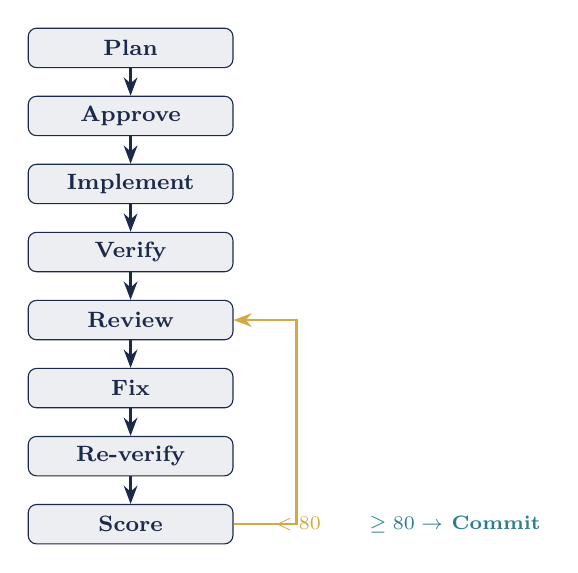
\begin{tikzpicture}[
  node distance=0.35cm,
  box/.style={
    rectangle, rounded corners=3pt,
    draw=NavyPrimary, fill=NavyPrimary!8,
    minimum width=2.6cm, minimum height=0.5cm,
    font=\footnotesize\bfseries, text=NavyPrimary,
    align=center
  },
  arr/.style={
    -Stealth, thick, NavyPrimary
  },
  loopstyle/.style={
    -Stealth, thick, GoldAlert
  }
]
  \node[box] (plan) {Plan};
  \node[box, below=of plan] (approve) {Approve};
  \node[box, below=of approve] (impl) {Implement};
  \node[box, below=of impl] (verify) {Verify};
  \node[box, below=of verify] (review) {Review};
  \node[box, below=of review] (fix) {Fix};
  \node[box, below=of fix] (reverify) {Re-verify};
  \node[box, below=of reverify] (score) {Score};

  \draw[arr] (plan) -- (approve);
  \draw[arr] (approve) -- (impl);
  \draw[arr] (impl) -- (verify);
  \draw[arr] (verify) -- (review);
  \draw[arr] (review) -- (fix);
  \draw[arr] (fix) -- (reverify);
  \draw[arr] (reverify) -- (score);

  % Loop arrow from Score back to Review
  \draw[loopstyle]
    (score.east) --
    ++(0.8,0) node[midway, right, font=\scriptsize,
      text=GoldAlert] {$<80$} |-
    (review.east);

  % Pass label
  \node[right=1.6cm of score,
    font=\scriptsize\bfseries,
    text=TealAccent] {$\geq 80 \to$ Commit};
\end{tikzpicture}
\end{center}

\end{frame}

% --- Slide 5: Limits and Just Do It Mode ---
\begin{frame}{Safeguards and Shortcuts}

\begin{columns}[T]
\column{0.48\textwidth}
\textbf{Built-in limits}
\begin{itemize}
  \item Main loop: max 5 review-fix rounds
  \item Critic-fixer sub-loop: max 5 rounds
  \item Verification retries: max 2 attempts
  \item Never loops indefinitely
\end{itemize}

\column{0.48\textwidth}
\textbf{``Just do it'' mode}

Triggered by \textit{``just do it''} or
\textit{``handle it''}:
\begin{itemize}
  \item Skips final approval pause
  \item Auto-commits if score $\geq 80$
  \item Still runs full verify-review-fix loop
\end{itemize}
\end{columns}

\begin{keybox}
The orchestrator is autonomous \emph{after}
plan approval---but always respects the
quality gate.
\end{keybox}

\end{frame}

% =====================================================================
% SECTION 3: Specialized Agents
% =====================================================================
\section{Specialized Agents}

% --- Slide 6: Eight Agents ---
\begin{frame}{Review Agents}

\begin{center}
\small
\begin{tabular}{@{}lll@{}}
\toprule
\textbf{Agent} & \textbf{Scope}
  & \textbf{Trigger} \\
\midrule
Proofreader & Grammar, typos, overflow
  & Any \texttt{.tex} \\
Slide Auditor & Layout, spacing, box fatigue
  & Beamer slides \\
Pedagogy Reviewer & Narrative, pacing, notation
  & Lecture decks \\
Domain Reviewer & Derivations, citations
  & Technical slides \\
TikZ Reviewer & Label positions, overlaps
  & TikZ diagrams \\
R Reviewer & Code quality, themes
  & \texttt{.R} scripts \\
Python Reviewer & Paths, seeds, docstrings
  & \texttt{.py} scripts \\
Stata Reviewer & Headers, logs, seeds
  & \texttt{.do} files \\
\bottomrule
\end{tabular}
\end{center}

\end{frame}

% --- Slide 7: Agent Selection ---
\begin{frame}{Agent Selection by File Type}

\begin{center}
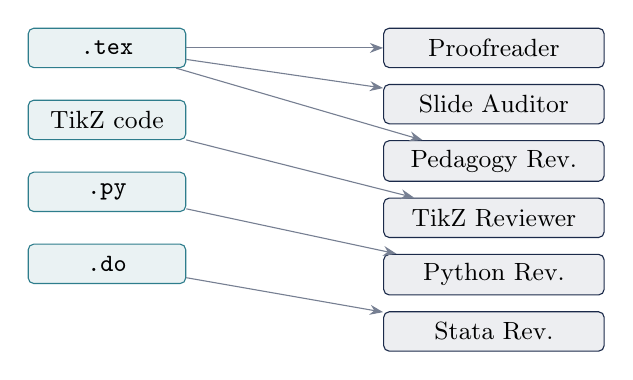
\begin{tikzpicture}[
  node distance=0.4cm and 2.5cm,
  filebox/.style={
    rectangle, rounded corners=2pt,
    draw=TealAccent, fill=TealAccent!10,
    minimum width=2cm, minimum height=0.5cm,
    font=\small, align=center
  },
  agentbox/.style={
    rectangle, rounded corners=2pt,
    draw=NavyPrimary, fill=NavyPrimary!8,
    minimum width=2.8cm, minimum height=0.5cm,
    font=\small, align=center
  },
  conn/.style={
    -Stealth, thin, NavyPrimary!60
  }
]
  % File types (left)
  \node[filebox] (tex) {\texttt{.tex}};
  \node[filebox, below=of tex] (tikz) {TikZ code};
  \node[filebox, below=of tikz] (py) {\texttt{.py}};
  \node[filebox, below=of py] (do) {\texttt{.do}};

  % Agents (right)
  \node[agentbox, right=of tex] (proof) {Proofreader};
  \node[agentbox, below=0.2cm of proof] (audit)
    {Slide Auditor};
  \node[agentbox, below=0.2cm of audit] (peda)
    {Pedagogy Rev.};
  \node[agentbox, below=0.2cm of peda] (tikzr)
    {TikZ Reviewer};
  \node[agentbox, below=0.2cm of tikzr] (pyrev)
    {Python Rev.};
  \node[agentbox, below=0.2cm of pyrev] (starev)
    {Stata Rev.};

  % Connections
  \draw[conn] (tex) -- (proof);
  \draw[conn] (tex) -- (audit);
  \draw[conn] (tex) -- (peda);
  \draw[conn] (tikz) -- (tikzr);
  \draw[conn] (py) -- (pyrev);
  \draw[conn] (do) -- (starev);
\end{tikzpicture}
\end{center}

\begin{highlightbox}
Specialization beats generalist review: each
agent applies domain-specific rubrics and catches
issues a general reviewer would miss.
\end{highlightbox}

\end{frame}

% =====================================================================
% SECTION 4: Quality Scoring
% =====================================================================
\section{Quality Scoring}

% --- Slide 8: Three Thresholds ---
\begin{frame}{Quality Thresholds}

\begin{center}
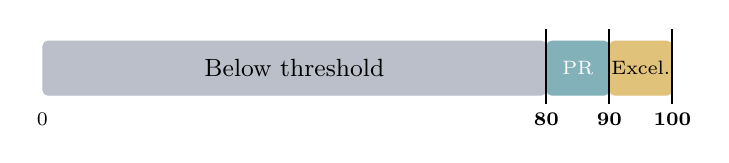
\begin{tikzpicture}[
  bar/.style={
    rectangle, minimum height=0.7cm,
    font=\small\bfseries, text=white,
    rounded corners=2pt
  }
]
  % Background bar (full width = 8cm for score 100)
  \fill[LightGray, rounded corners=2pt]
    (0,0) rectangle (8,0.7);

  % Commit zone: 0--80 (scaled: 0--6.4)
  \fill[NavyPrimary!30, rounded corners=2pt]
    (0,0) rectangle (6.4,0.7);

  % PR zone: 80--90 (scaled: 6.4--7.2)
  \fill[TealAccent!60, rounded corners=2pt]
    (6.4,0) rectangle (7.2,0.7);

  % Excellence zone: 90--100 (scaled: 7.2--8)
  \fill[GoldAlert!70, rounded corners=2pt]
    (7.2,0) rectangle (8,0.7);

  % Labels
  \node at (3.2,0.35) [font=\small] {Below threshold};
  \node at (6.8,0.35) [font=\scriptsize, text=white]
    {PR};
  \node at (7.6,0.35) [font=\scriptsize] {Excel.};

  % Tick marks
  \draw[thick] (6.4,-0.1) -- (6.4,0.85);
  \node[below, font=\scriptsize\bfseries] at (6.4,-0.1)
    {80};

  \draw[thick] (7.2,-0.1) -- (7.2,0.85);
  \node[below, font=\scriptsize\bfseries] at (7.2,-0.1)
    {90};

  \draw[thick] (8,-0.1) -- (8,0.85);
  \node[below, font=\scriptsize\bfseries] at (8,-0.1)
    {100};

  \node[below, font=\scriptsize] at (0,-0.1) {0};
\end{tikzpicture}
\end{center}

\vspace{0.3cm}

\begin{tabular}{@{}cll@{}}
\toprule
\textbf{Score} & \textbf{Gate}
  & \textbf{Meaning} \\
\midrule
$\geq 80$ & Commit
  & Good enough to save \\
$\geq 90$ & Pull Request
  & Ready for deployment \\
$\geq 95$ & Excellence
  & Aspirational target \\
\bottomrule
\end{tabular}

\end{frame}

% --- Slide 9: Deduction Examples ---
\begin{frame}{How Scores Are Calculated}

Each file type starts at 100 and loses points for detected issues.

\vspace{0.2cm}
\begin{columns}[T]
\column{0.30\textwidth}
\textbf{LaTeX deductions}
\begin{tabular}{@{}lr@{}}
\toprule
Issue & Pts \\
\midrule
Compile fail & 100 \\
Bad citation & $-15$ \\
Overfull hbox & $-10$ \\
Text overflow & $-5$ \\
Notation & $-3$ \\
\bottomrule
\end{tabular}

\column{0.30\textwidth}
\textbf{Python deductions}
\begin{tabular}{@{}lr@{}}
\toprule
Issue & Pts \\
\midrule
Syntax error & 100 \\
Hard path & $-20$ \\
No import & $-10$ \\
No seed & $-10$ \\
No docstring & $-5$ \\
\bottomrule
\end{tabular}

\column{0.30\textwidth}
\textbf{Stata deductions}
\begin{tabular}{@{}lr@{}}
\toprule
Issue & Pts \\
\midrule
Syntax error & 100 \\
Hard path & $-20$ \\
No clear & $-10$ \\
No seed & $-10$ \\
No log & $-5$ \\
\bottomrule
\end{tabular}
\end{columns}

\end{frame}

% =====================================================================
% SECTION 5: Configuration Layers
% =====================================================================
\section{Configuration Layers}

% --- Slide 10: Five Layers ---
\begin{frame}{Configuration Stack}

\begin{center}
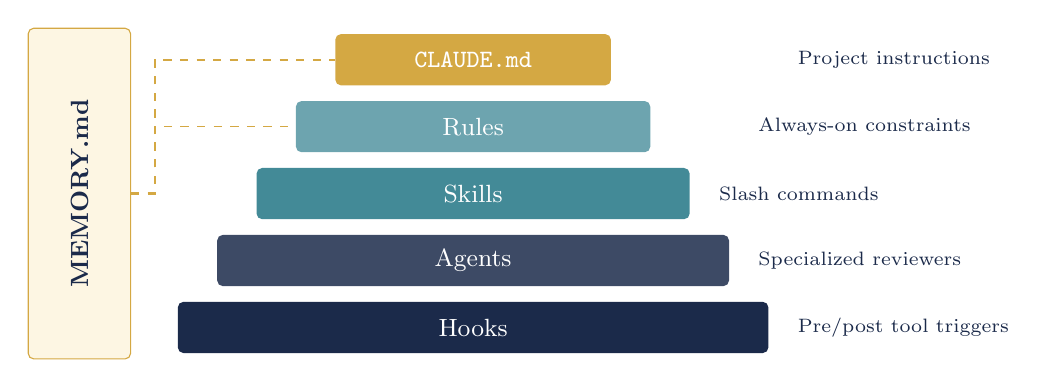
\begin{tikzpicture}[
  layer/.style={
    rectangle, rounded corners=2pt,
    minimum height=0.65cm,
    font=\small, align=center,
    text=white
  },
  note/.style={
    font=\scriptsize, text=NavyPrimary,
    align=left
  }
]
  % Stacked bars (bottom to top)
  \node[layer, fill=NavyPrimary,
    minimum width=7.5cm] (hooks)
    at (0,0) {Hooks};
  \node[layer, fill=NavyPrimary!85,
    minimum width=6.5cm] (agents)
    at (0,0.85) {Agents};
  \node[layer, fill=TealAccent!90,
    minimum width=5.5cm] (skills)
    at (0,1.70) {Skills};
  \node[layer, fill=TealAccent!70,
    minimum width=4.5cm] (rules)
    at (0,2.55) {Rules};
  \node[layer, fill=GoldAlert,
    minimum width=3.5cm] (claude)
    at (0,3.40) {\texttt{CLAUDE.md}};

  % Descriptions on the right
  \node[note, right] at (4.0,3.40)
    {Project instructions};
  \node[note, right] at (3.5,2.55)
    {Always-on constraints};
  \node[note, right] at (3.0,1.70)
    {Slash commands};
  \node[note, right] at (3.5,0.85)
    {Specialized reviewers};
  \node[note, right] at (4.0,0)
    {Pre/post tool triggers};

  % Memory sidebar
  \node[rectangle, rounded corners=2pt,
    draw=GoldAlert, fill=LightGold,
    minimum width=1.3cm, minimum height=4.2cm,
    font=\small, align=center,
    text=NavyPrimary] (mem) at (-5,1.70)
    {\rotatebox{90}{\textbf{MEMORY.md}}};

  \draw[dashed, GoldAlert, thick]
    (mem.east) -- ++(.3,0) |- (claude.west);
  \draw[dashed, GoldAlert]
    (mem.east) -- ++(.3,0) |- (rules.west);
\end{tikzpicture}
\end{center}

\end{frame}

% --- Slide 11: Always-On vs Path-Scoped ---
\begin{frame}{Rules: Always-On vs.\ Path-Scoped}

\begin{columns}[T]
\column{0.48\textwidth}
\begin{definitionbox}[Always-On Rules]
Loaded every session, regardless of task.

Examples:
\begin{itemize}
  \item Plan-first workflow
  \item Session logging protocol
  \item Quality gate enforcement
  \item Orchestrator protocol
\end{itemize}
\end{definitionbox}

\column{0.48\textwidth}
\begin{definitionbox}[Path-Scoped Rules]
Activated only when editing matching file paths.

Examples:
\begin{itemize}
  \item \texttt{slides/*.tex} $\to$ Beamer rules
  \item \texttt{scripts/python/} $\to$ Python rules
  \item \texttt{stata/} $\to$ Stata conventions
\end{itemize}
\end{definitionbox}
\end{columns}

\vspace{0.3cm}

\begin{keybox}
Path scoping keeps the agent's context focused:
it only loads rules relevant to the current task.
\end{keybox}

\end{frame}

% =====================================================================
% SECTION 6: Project Workflow
% =====================================================================
\section{Project Workflow}

% --- Slide 12: Clone-Per-Project ---
\begin{frame}[fragile]{Clone-Per-Project Setup}

Each research project gets its own clone of the workflow template.

\vspace{0.2cm}
\begin{highlightbox}
\begin{enumerate}
  \item Clone the workflow repo
  \item Rename \texttt{origin} to \texttt{workflow}
  \item Add project-specific \texttt{origin} remote
  \item Customize \texttt{CLAUDE.md} for the project
\end{enumerate}
\end{highlightbox}

\vspace{0.2cm}
\begin{lstlisting}
git clone <workflow-repo> my-project
cd my-project
git remote rename origin workflow
git remote add origin <project-repo>
git push -u origin main
\end{lstlisting}

The \texttt{workflow} remote stays connected for pulling infrastructure updates.

\end{frame}

% --- Slide 13: Sync Script ---
\begin{frame}[fragile]{Syncing Infrastructure Updates}

\texttt{sync-workflow.sh} propagates infrastructure
changes without overwriting project-specific content.

\vspace{0.2cm}
\begin{columns}[T]
\column{0.48\textwidth}
\textbf{Synced (infrastructure)}
\begin{itemize}
  \item \texttt{.claude/} rules, skills, hooks
  \item \texttt{scripts/quality\_score.py}
  \item \texttt{templates/}
  \item \texttt{preambles/header.tex}
\end{itemize}

\column{0.48\textwidth}
\textbf{Never synced (project)}
\begin{itemize}
  \item \texttt{CLAUDE.md} (customized)
  \item \texttt{slides/}, \texttt{data/}
  \item \texttt{scripts/python/} analysis
  \item \texttt{stata/} scripts
\end{itemize}
\end{columns}

\vspace{0.2cm}
\begin{lstlisting}
# Usage
./scripts/sync-workflow.sh /path/to/project
\end{lstlisting}

\end{frame}

% =====================================================================
% SECTION 7: Research Workflows
% =====================================================================
\section{Research Workflows}

% --- Slide 14: Exploration Sandbox ---
\begin{frame}{Exploration Sandbox}

Fast experimentation without full plan overhead.

\vspace{0.2cm}
\begin{columns}[T]
\column{0.48\textwidth}
\begin{definitionbox}[Fast-Track]
For quick tests and prototypes:
\begin{itemize}
  \item Work in \texttt{explorations/}
  \item No plan required
  \item Date-prefixed files
  \item Lightweight logging
\end{itemize}
\end{definitionbox}

\column{0.48\textwidth}
\begin{definitionbox}[Plan-First]
For production-bound work:
\begin{itemize}
  \item Full plan approval
  \item Orchestrator loop
  \item Quality gates enforced
  \item Session log required
\end{itemize}
\end{definitionbox}
\end{columns}

\vspace{0.2cm}

Explorations that prove useful get promoted to
\texttt{scripts/} or \texttt{slides/} via the
standard plan-first workflow.

\end{frame}

% --- Slide 15: Research Skills ---
\begin{frame}{Built-In Research Skills}

Slash commands for common research tasks:

\vspace{0.2cm}
\begin{center}
\small
\begin{tabular}{@{}ll@{}}
\toprule
\textbf{Command} & \textbf{What It Does} \\
\midrule
\texttt{/lit-review [topic]}
  & Literature search + synthesis \\
\texttt{/research-ideation [topic]}
  & Research questions + strategies \\
\texttt{/interview-me [topic]}
  & Interactive research interview \\
\texttt{/review-paper [file]}
  & Manuscript review \\
\texttt{/data-analysis [dataset]}
  & End-to-end Python/Stata analysis \\
\texttt{/slide-excellence [file]}
  & Combined multi-agent review \\
\bottomrule
\end{tabular}
\end{center}

\vspace{0.1cm}

\begin{highlightbox}
Each skill is a structured prompt that orchestrates
tools, agents, and verification steps into
repeatable workflows.
\end{highlightbox}

\end{frame}

% =====================================================================
% CLOSING
% =====================================================================
\section{Summary}

% --- Slide 16: Five Key Takeaways ---
\begin{frame}{Key Takeaways}

\begin{enumerate}
  \item \faClipboardCheck\hspace{4pt}
    \textbf{Plan first} ---
    every non-trivial task starts with a plan

  \item \faCogs\hspace{4pt}
    \textbf{Specialized agents} ---
    domain-specific review beats generalist

  \item \faChartBar\hspace{4pt}
    \textbf{Quality gates} ---
    80/90/95 thresholds enforce standards

  \item \faLayerGroup\hspace{4pt}
    \textbf{Layered config} ---
    CLAUDE.md, rules, skills, agents, hooks

  \item \faSync\hspace{4pt}
    \textbf{Clone and sync} ---
    one template, many projects, easy updates
\end{enumerate}

\end{frame}

% --- Slide 17: Resources ---
\begin{frame}{Getting Started}

\begin{columns}[T]
\column{0.55\textwidth}
\textbf{Quick start}
\begin{enumerate}
  \item Clone the workflow repo
  \item Run \texttt{git remote rename origin workflow}
  \item Add your project remote
  \item Customize \texttt{CLAUDE.md}
  \item Start with \texttt{/create-lecture} or
        \texttt{/data-analysis}
\end{enumerate}

\column{0.40\textwidth}
\textbf{Resources}
\begin{itemize}
  \item Workflow guide:\\
    {\small\texttt{guide/workflow-guide.md}}
  \item Template repo:\\
    {\small\texttt{etjernst/claude-code-}}\\
    {\small\texttt{my-workflow}}
  \item Claude Code docs:\\
    {\small\texttt{docs.anthropic.com}}
\end{itemize}
\end{columns}

\vspace{0.3cm}
\begin{keybox}
The workflow is designed to be forked and customized.
Start with the defaults, then adapt the rules
and agents to your research domain.
\end{keybox}

\end{frame}

\end{document}
